
Given F(X) is the CDF of the random variable $X$.
\\$P(2\le X<4)$ will be the sum of all the probabilities of values the random variable $X$ can take in $[2,4)$.
\\So it is the difference between CDF values of the random variable X at X=4- and at X=2-.
\\Therefore,
\begin{align}
P(2\le X<4)&=\lim_{X \to 4-}{F(X)}-\lim_{X \to 2-}{F(X)}
 \\     &= \lim_{X \to 4-}{1}-\lim_{X \to 2-}{\frac{3}{5}}
 \\ &= 1-\frac{3}{5}
 \\ &=\frac{2}{5}=0.4
\end{align}
Hence,$P(2\le X<4) = 0.4$.\begin{figure}[ht]
    \centering
    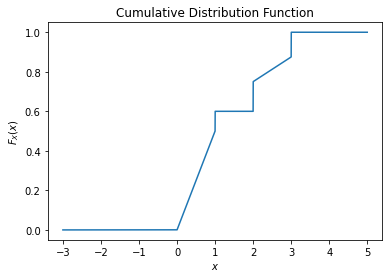
\includegraphics[width=\columnwidth]{solutions/ec/58/CDF.png}
    \caption{CDF of X}
    \label{fig:my_label}
\end{figure}

